

\author[Niklas Brunn]{Nix}


\beamertemplatenavigationsymbolsempty{}

\logo{
\includegraphics[height=1cm]{Bilder/logo}}



\section{ODE$^{2}$VAE}

\begin{frame}
    \frametitle{ODE$^{2}$VAE}
    Paper: \emph{ODE$^{\ 2}$VAE: Deep generative second order ODEs with Bayesian neural networks} von Ç. Yıldız, M. Heinonen und H. Lähdesmäki.
\end{frame}




\begin{frame}
	\frametitle{Idee}
	\begin{itemize}
	\item Bewegungen (z.B. rot.MNIST) lassen sich nicht gut mit einem Standard-VAE modellieren\\
	\item neuer Ansatz: Zeitliche Abhängigkeit der Daten berücksichtigen und die Bewegung durch Differentialgleichungen zweiter Ordnung (ODE$^{2}$) erlernen 
	\item Vorteile: Wir können so zu beliebigen Zeitpunkten abfragen und auch Prognosen für die Zukunft generieren
	\end{itemize}
\end{frame}



\begin{frame}
    \frametitle{Modell}
    \begin{itemize}
    	\item Datensatz $\mathbf{x}_{0:T}=(\mathbf x_{0}, \mathbf x_{1}, \ldots,\mathbf x_{T})\in \mathbb{R}^{D\times T}$ zu beobachtete Zeitpunkten $t_{0}, t_{1},\ldots,t_{T}$\\
    	\item Annahme: Zeitliche Änderung kann stetig durch eine ODE$^{2}$ beschrieben werden\\
    	\item Zugehörigen latenten Zustände sind $\mathbf z_{0:T}=(\mathbf z_{0}, \mathbf z_{1}, \ldots, \mathbf z_{T})\in \mathbb{R}^{d\times T}$\\ 
    	\item Latente Zustände werden in Positions- und Geschwindigkeitskomponente aufgeteilt $\mathbf z_{t}=(\mathbf s_{t}, \mathbf v_{t})$
    \end{itemize}
\end{frame}




\begin{frame}
\frametitle{Modell}
    \begin{itemize}
    	\item Die ODE$^{2}$ lässt sich als ein System zweier ODE$^{1}$ schreiben\\
    	\item $f_{\boldsymbol{\psi}}$ ist dabei ein NN, welches die Beschleunigungskurve erlernt
    	\item Lösen des Anfangswertproblems in $\mathbf{z}_{0}=(\mathbf{s}_{0}, \mathbf{v}_{0})$ liefert zu beliebigen Zeitpunkten $T$ eine Lösung
	\end{itemize}
    {\footnotesize\begin{align*}
    \dfrac{\partial^2 \mathbf{z}(t)}{\partial^2 t}&=f_{\boldsymbol{\psi}}\left(\mathbf{z}(t), \tfrac{\partial \mathbf{z}(t)}{\partial t}, t\right), \\
    \begin{cases*}
    \tfrac{\partial \mathbf{s}(t)}{\partial t}=\mathbf v(t) \\
    \tfrac{\partial \mathbf{v}(t)}{\partial t}=f_{\boldsymbol{\psi}}(\mathbf s(t), \mathbf v(t), t) \\
    \end{cases*},
    \left(\begin{array}{cc}
    \mathbf s_{T} \\
    \mathbf v_{T}
    \end{array}\right)
    &=
    \left(\begin{array}{cc}
    \mathbf s_{0} \\
    \mathbf v_{0}
    \end{array}\right)
    +
    \int_{0}^{T}
    \left(\begin{array}{cc}
    \mathbf v(t) \\
    f_{\boldsymbol{\psi}}(\mathbf s(t), \mathbf v(t), t)
    \end{array}\right)
    \mathrm{d}t.
    \end{align*}}
\end{frame}




\begin{frame}
\frametitle{Modell}
Das Modell besteht aus den folgenden Komponenten:
\begin{itemize}
	\item Einer Standardnormalverteilung $\mathcal{N}(\mathbf{0},\mathbf{I})$ für die latenten Werte
	\item Einem \emph{Position-Encoder} welcher mit $\mathbf{x}_{0}$ die erste latente Ausgangsposition $\mathbf{s}_{0}$ encodiert und einem \emph{Velocity-Encoder} welcher mit den ersten $m\geq2$ Werten $\mathbf{x}_{m}$ die latente Ausgangsgeschwindigkeit encodiert\\
    \item Einem \emph{ODE-Netzwerk}\footnote{im Paper wird ein Bays-Net vorgestellt, wir bleiben bei einem NN} um welches zu einem Anfangswert eine Kurve im latenten Raum bestimmt\\
    \item Einem Decoder, welcher die aus der Kurve resultierenden latenten Positionen decodiert
\end{itemize}
\end{frame}




\begin{frame}
    \frametitle{Modell}
    	\begin{figure}[h!]
    	\centering
    	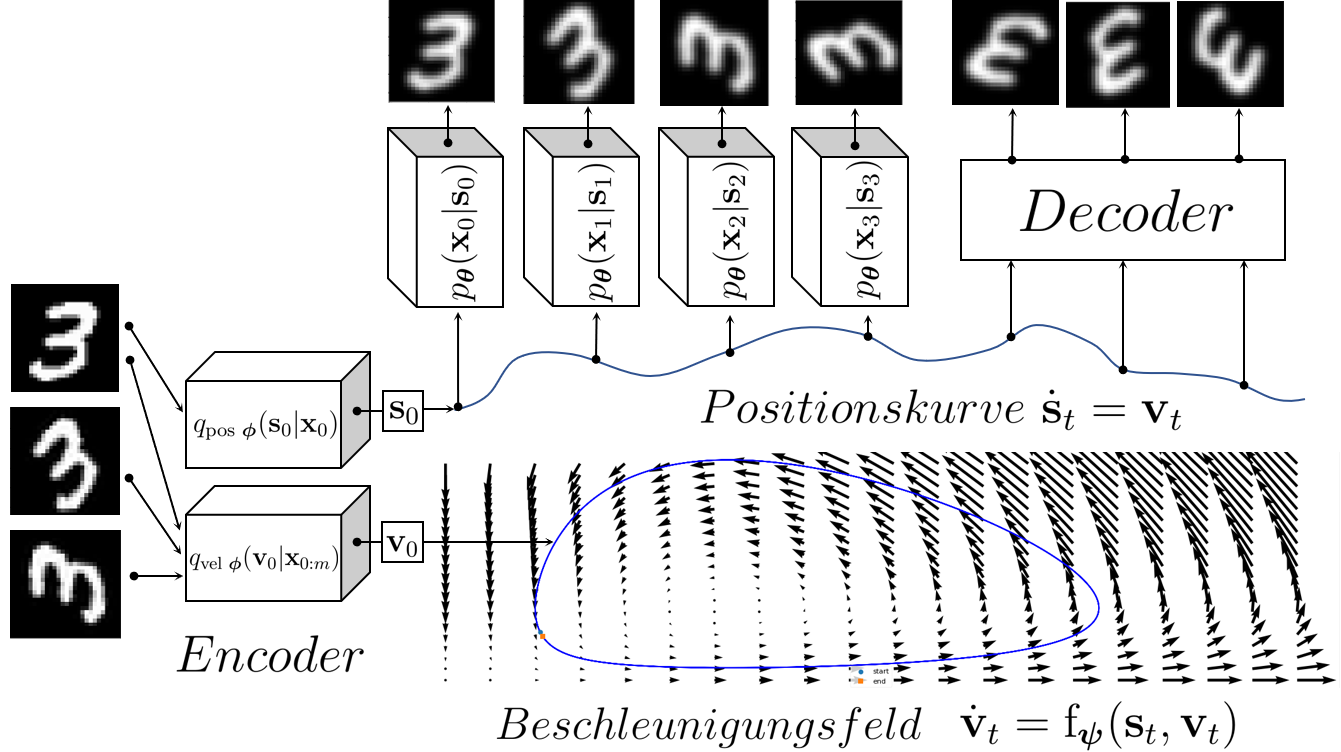
\includegraphics[scale=0.36]{Bilder/ODE2VAE_ODE_Net}
    \end{figure}
\end{frame}




\begin{frame}
    \frametitle{Training}
    Als Trainingskriterium verwenden wir die negative ELBO \footnote{Für Details siehe schriftliche Ausarbeitung und Code auf GitHub %wir verwenden eine eicht abgewandelte aber ähnliche Version der Lossfunktion}
    }	
    	{\footnotesize\begin{align*}
    \log\big(p_{\boldsymbol{\theta}}(\mathbf{x}_{0:T})\big)&\ge \E_{\mathbf{z}_{0:T}\sim q_{\boldsymbol\phi,\boldsymbol\psi}}
    \left[\log\big(p_{\boldsymbol\theta}\left(\mathbf{x}_{0:T}|\mathbf{z}_{0:T}\right)\big)\right] - D_{KL}\big[q_{\boldsymbol\phi,\boldsymbol\psi}(\mathbf{z}_{0:T}|\mathbf{x}_{0:m})||p_{\boldsymbol\theta,\boldsymbol\psi}(\mathbf{z}_{0:T})\big]\\
    &=\underbrace{\E_{\mathbf{z}_{0}\sim q_{\text{enc }\boldsymbol\phi}}
    	\left[\log\big(p_{\boldsymbol\theta}\left(\mathbf{x}_{0}|\mathbf{z}_{0}\right)\big)\right] - D_{KL}\big[q_{\text{enc }\boldsymbol\phi}(\mathbf{z}_{0}|\mathbf{x}_{0:m})||p_{\boldsymbol\theta}(\mathbf{z}_{0})\big]}_{\text{Vanilla-VAE ELBO}}\\ &+ \underbrace{\sum_{t=1}^T \E_{\mathbf{z}_{t}\sim q_{\text{ode }\boldsymbol\psi}}
    	\left[\log\big(p_{\boldsymbol\theta}\left(\mathbf{x}_{t}|\mathbf{z}_{t}\right)\big)\right] - D_{KL}\big[q_{\text{ode }\boldsymbol\psi}(\mathbf{z}_{t}|\mathbf{x}_{0:m})||p_{\boldsymbol\theta,\boldsymbol\psi}(\mathbf{z}_{t})\big]}_{\text{dynamic loss}}
    \end{align*}}
\end{frame}


%\begin{frame}
    %\frametitle{ODE$^{2}$VAE}
    %Inhalt
%\end{frame}
